%!TeX root = ./../Bachelorarbeit.tex

%##########################################################
% Inhalt
%##########################################################

\clearpage

\chapter{Implementation}

\section{QEMU Device Erweiterung}

Wie in \ref{konzept-qemu-dev} beschrieben werden Peripherie und Mikrocontroller
in QEMU durch verschiedene \acp{api} integriert.
QEMU implementiert mithilfe der \ac{qom}- und \ac{qdev}-\acp{api} einen
Objektorientierten Ansatz.
Da C keine Objektorientierte Programmiersprache ist und nur ein vergleichsweise
minimales Typsystem unterstützt werden in QEMU viele dieser Konzepte mittels
Makro-Programmierung\footnotemark[1] realisiert.
\newline
Jede Maschine und jede Peripherie in QEMU ist ein Objekt einer Klasse.
Moderne Klassen in QEMU sollten von der \texttt{TYPE\_SYS\_BUS\_DEVICE} Klasse
erben.
Vom Typ \texttt{TYPE\_SYS\_BUS\_DEVICE} erbende Objekte werden im Falle eines
Reset-Events automatisch zurückgesetzt.
Das Reset-Event und Resettable-Interface werden in Kapitel
\ref{sec:impl-qemu-reset} erklärt.
Die Details der Instanziierung einer Klasse werden in Kapitel
\ref{sec:impl-qemu-device-build-obj} erläutert.
\newline
Nach Aufstart von QEMU wird als Erstes die Maschine erzeugt.
Welche Maschine gestartet werden soll wird durch den Kommandozeilenbefehl
\texttt{-machine/-M} ausgewählt.
Die Maschine erstellt \ac{cpu} und \ac{soc}, welcher anschließend für die
Realisierung der Peripherie zuständig ist.
So ensteht eine Baum-Hierarchie, welche in QEMU auch \enquote{QOM-tree} genannt
wird.
Im QOM-tree sind alle Objekte einer Maschine repräsentiert.
\newline
Im ersten Schritt werden die Quelldateien dem Build-System hinzugefügt.
Für eine bessere Abgrenzung wird die neue Maschine
\texttt{stm32f429-thesis-device} erstellt, welche das \enquote{Testboard} in
QEMU darstellen soll.

\subsection{Build-Konfiguration und Objekt Erstellung}
\label{sec:impl-qemu-device-build-obj}

Um eine neue ARM Maschine zu registrieren muss die Konfiguration der
\textbf{Kconfig}\footnotemark[2] Datei im ARM Verzeichnis angepasst werden.
QEMU erstellt für die Emulation jeder unterstützten Architektur ein
individuelles Binary, beispielsweise \texttt{qemu-system-arm} oder
\texttt{qemu-system-x86}.
Mittels Kconfig und Meson wird sichergestellt das Quelldateien nur für die
vorgesehenen Architekturen in das jeweilige Programm gelinkt werden.
Ein Kconfig-Eintrag besteht aus der Definition selbst und einer variablen
Anzahl an Modulen die eingebunden werden.

% Makro-Programmierung Footnote
\footnotetext[1]{In C werden Textmakros vor der Übersetzung vom
Präprozessor ersetzt.}
% Kconfig Erklärung Footnote
\footnotetext[2]{Kconfig entstandt ursprünglich im Linux-Kernel Projekt und
wird in QEMU zur Verwaltung der Abhängigkeiten verwendet\cite{QemuDocsKconfig}.}

\begin{minipage}{\linewidth}
\lstinputlisting[language=,numbers=none,
                label={lst:qemu-kconfig},
                linerange={157-162,467-478},
                caption=ARM Kconfig Konfiguration von Maschine und \ac{soc}]
                {anlagen/qemu-device/KConfig.config}
\end{minipage}

Für die Einbindung des Mikrocontrollers werden in \ref{lst:qemu-kconfig} die
Konfigurationen für den \ac{soc} und die Maschine hinzugefügt.
Die Maschine benötigt das \ac{tcg} und ARM Modul.
Mit \texttt{select} wird der STM32F429-\ac{soc} der Maschine hinzugefügt und
beim Build-System registriert.
In der Konfiguration des \ac{soc} wird anschließend ausgewählt, welche
Peripherie und welcher Mikroprozessor verwendet werden soll.
Im Falle des STM32F429 ist ein ARM Cortex-M4 Mikroprozessor verbaut, welcher
auf der ARM-V7M Architektur basiert.
Als Vorlage für die Maschine wurde das bereits in QEMU implementierte
\textbf{olimex-stm32-h405} Entwicklungsboard verwendet\cite{QemuOlimexBoard}.
Die Grundlage für den STM32F429-\ac{soc} bildet der vom Olimex-Board verwendete
STM32F405-\ac{soc}\cite{QemuStmF405Soc}.
\newline
In \ref{lst:qemu-soc-header} wird der State für den STM32F429-\ac{soc} als
\texttt{struct} deklariert.
Hier erfolgt auch die Deklaration des STM32F429-\ac{soc} Typs.
Er implementiert die unterschiedlichen Peripherie-Devices, Speicherregionen,
sowie System- und Referenz Takt.
Für STM32F4 und STM32F2 Mikrocontroller existieren bereits unterschiedliche
Peripherien.
In der QEMU Dokumentation wird beschrieben, dass die Produktfamilien STM32F4
und STM32F2 Pin kompatibel sind.
Es können also auch Peripherie Implementationen für Mikrocontroller der
STM32F2-Familie verwendet werden.
Die Peripherie wird später während der \ac{soc}-Realisierung als \enquote{QEMU
Device} erstellt und dem QOM-tree hinzugefügt.
\newline
Tabelle \ref{tab:stm32-memory} zeigt die verschiedenen Speichertypen des
STM32F429-\ac{soc}.
Die Daten sind im STM32-\ac{trm} Sektion 3.4 für Flash-Speicher und Sektion
2.3.1 für \ac{sram} und \ac{ccm} definiert\cite{Stm32F4Trm}.
Die Speicherregionen werden ebenfalls während der Initialisierung des \ac{soc}
realisiert.

\begin{table}[h!]
    \centering
    \caption{Speichertypen mit Größe und Startadresse im 32-Bit-Adressraum}
    \label{tab:stm32-memory}
    \begin{tabular}{||P{3cm}|P{5cm}|P{4cm}||}
        \hline
        \textbf{Speichertyp} & \textbf{Speichergröße in KB} & \textbf{Startadresse} \\
        \hline
        \hline
        \hspace{0.8cm}
        Flash & 2048 & 0x0800 0000 \\
        \hline
        \hspace{0.8cm}
        \ac{sram} & 256 & 0x2000 0000 \\
        \hline
        \hspace{0.8cm}
        \ac{ccm} & 64 & 0x1000 0000 \\
        \hline
    \end{tabular}
\end{table}

Um die Maschine in der Kommandozeilenanwendung auszuwählen, muss diese
allerdings erst noch als statischer Typ registriert werden.
Die Registrierung einer Maschine unterscheidet sich leicht von der eines
Devices.
In \ref{lst:qemu-machine-init} erfolgt die Registrierung der neuen Maschine.
Das Makro \texttt{DEFINE\_MACHINE} registriert die Maschine als statischen Typ.
Anders als bei einem Device ist die Basisklasse einer Maschine
\texttt{MACHINE\_TYPE}.
Die Methode \texttt{stm32\_f429\_thesis\_machine\_init} ist verantwortlich für
die \enquote{oberflächliche} Initialisierung der Maschine.
Falls vorhanden können hier Argumente verarbeitet werden, die bei Aufstart von
QEMU über die Kommandozeile Argumente übergeben wurden.
Des Weiteren enthält sie die Beschreibung der Maschine, sowie die konkrete
Initialisierung durch die \texttt{stm32\_f429\_thesis\_init} Methode.
In der konkreten Initialisierung werden Mikroprozessor und \ac{soc} erstellt.
Da alle STM32F429 Mikrocontroller den Cortex-M4 Mikroprozessor wird nur dieser
erlaubt.
Sowohl für Maschinen als auch normale Devices existieren eine Methode zur
Initialisierung der Klasse, und eine Methode zur Initialisierung des Objekts.
Eine \texttt{class\_init} Methode wird immer vor Aufruf der Objekt
Initialisierung ausgeführt.

\begin{minipage}{\linewidth}
\lstinputlisting[language=c,numbers=none,
                label={lst:qemu-machine-init},
                linerange={36-51},
                caption=Initialisierung und Registrierung der STM32F429-thesis Maschine]
                {anlagen/qemu-device/stm32f429_thesis.c}
\end{minipage}

\subsection{GPIO-Peripherie des STM32F429}

Wie in \ref{sec:concept-periphery-selection} erwähnt soll das \ac{gpio}-Module
implementiert werden.
Die Konfiguration des Build-Systems erfolgt analog zur Implementation der
Maschine und des \ac{soc}.
Es müssen die Kconfig und Meson Konfiguration im \ac{gpio}-Peripherie Verzeichnis
angepasst werden.
Jeder \ac{gpio} Port wird als ein eigenständiges Device modelliert.
In \ref{lst:qemu-gpio-header} wird der State für das \ac{gpio} Device erneut als
\texttt{struct} deklariert.
Alle Register sind 32-Bit breit und können als vorzeichenlose 32-Bit Ganzzahlen
dargestellt werden.
\newline
Aufgrund hoher Komplexität und fehlender Peripherie des STM32F429 in QEMU
können nicht alle Funktionalitäten des \ac{gpio} Moduls abgebildet werden.
Die \enquote{alternative Funktion}\footnotemark[3] und die Regulierung der
Eingabe-/Ausgabe-Frequenz eines \ac{gpio} Pins werden nicht unterstützt.
Es fehlen beispielsweise Unterstützung für Ethernet- und \ac{can}, sowie die
Implementation der \ac{rcc}-Peripherie.
% Alternate Function Footnote
\footnotetext[3]{english: alternate function}
In \ref{lst:qemu-gpio-memops} wird die Speicherregion während der
Initialisierung des Objekts initialisiert und dem Systembus bekannt gemacht.
Auf dem Systembus werden die meisten Peripherie Devices registriert.
In QEMU können jeder Speicherregion bestimmte Eigenschaften zugewiesen werden.
Dies erfolgt über ein Objekt des Typs \texttt{MemoryRegionOps}.
In diesem Objekt können verschiedene Eigenschaften bestimmt werden.
Lese- und Schreibzugriff auf die \ac{mmio}-Region (bzw. die Register) werden
über die Funktionen \texttt{stm32f429\_gpio\_read} und
\texttt{stm32f429\_gpio\_write} realisiert.
Diese werden als \enquote{Callbacks} registriert.
Es wird ebenfalls die Byte-Reihenfolge, sowie die erlaubte Größe eines Lese-
oder Schreibzugriffs festgelegt.
\newline
Um die Komplexität der \enquote{write}-Funktion zu verringern wird nur
ein 4 Byte (32-Bit) Zugriff erlaubt.
Damit werden umständliche und fehleranfällige Bit-Manipulationen unnötig.
Jedes Register des \ac{gpio}-Moduls hat einen individuellen Offset.
Dieser Offset kann in Sektion 8.4 des \ac{trm} für jedes Register nachgelesen
werden\cite{Stm32F4Trm}.
Sowohl der write- als auch der read-Funktion wird ein Offset Wert als Parameter
übergeben.
Der Offset in die \ac{mmio}-Speicherregion errechnet sich nach der simplen Formel
\ref{eq:qemu-gpio-mmio-offset}.
In beiden Funktionen kann dann mittels einer \texttt{switch-case} Anweisung des
\texttt{Offset\_\ac{mmio}} der Zugriff auf das jeweilige Register bestimmt
werden.
Bei einem Schreibzugriff wird der Funktion darüber hinaus noch ein Schreibwert
übergeben, der in das Register geschrieben wird.
\begin{equation}
    Offset_{\ac{mmio}} = Basisadresse_{\ac{mmio}} + Offset_{Parameter}
    \label{eq:qemu-gpio-mmio-offset}
\end{equation}
Sowohl bei lesendem, als auch bei schreibendem Zugriff kann je nach Register
der Status des \texttt{LCKR}-Registers aktualisiert werden.

Das \ac{gpio}-Modul des STM32F429 kann durch eine bestimme Sequenz an Schreib- und
Lesezugriffen auf das \texttt{LCKR}-Register die
Konfigurationsregister\footnotemark[4] \enquote{einfrieren}.
Diese Sequenz kann der Sektion 8.4.8 des \ac{trm} entnommen werden\cite{Stm32F4Trm}.
Der Pseudocode \ref{alg:qemu-device-lckr} erläutert den groben Ablauf der
Lock-Sequenz Implementation im \ac{gpio} State.
Die Sequenz besteht aus drei Schreib- und einem Lesezugriff, welche
nacheinander ausgeführt werden müssen.
Bei jedem Schreibzugriff müssen Bits 0 bis 16 gleichzeitig gesetzt werden.
Ein Zugriff auf das \texttt{LCKR}-Register ist daher nur als 32 Bit Zugriff
möglich.
Wird die Reihenfolge der Zugriffe nicht eingehalten, wird die Sequenz
abgebrochen und muss von neuem gestartet werden.
Nach Schritt 4, dem Lesezugriff, wird die Lock-Konfiguration angewendet.
Für jedes gesetzte Bit der Lock-Konfiguration\footnotemark[5] können die
korrespondierenden Bits in den Konfigurationsregistern nicht mehr geändert
werden.
\begin{algorithm}
    \floatname{algorithm}{Algorithmus}
    \caption{\texttt{LCKR}-Register Lock-Sequenz der Konfigurationsregister der
            \ac{gpio} Pins}
    \label{alg:qemu-device-lckr}
    \begin{algorithmic}[1]
        \State \textbf{Write} $lckr$ \gets \textbf{Set} $lckr[16]$ + $lckr[0..15]$
        \Comment{lckr[16] ist der Lock Schlüssel}
        \State \textbf{Write} $lckr$ \gets \textbf{Reset} $lckr[16]$ + $lckr[0..15]$
        \State \textbf{Write} $lckr$ \gets \textbf{Set} $lckr[16]$ + $lckr[0..15]$
        \State \textbf{Read} $lckr$
    \end{algorithmic}
\end{algorithm}

Die Lock-Konfiguration kann bis zum \textit{Reset} des Mikrocontrollers
nicht mehr geändert werden.
% Konfigurationsregister Footnote
\footnotetext[4]{Die Konfigurationsregister sind \texttt{MODER},
\texttt{OTYPER}, \texttt{PUPDR} und \texttt{OSPEEDR}.}
% LCKR Konfiguration Footnote
\footnotetext[5]{Die Lock-Konfiguration der \ac{gpio} Pins ist in den Bits 0
bis 15 des \texttt{LCKR} Registers enthalten.}
\newline
Die Implementation in QEMU wird in \ref{lst:qemu-gpio-lckr-write} exemplarisch
für den ersten Schritt der Sequenz dargestellt.
Bei einem Lese- oder Schreibzugriff auf das \texttt{LCKR}-Register wird die
Funktion \texttt{update\_lckr} ausgeführt.
Die Funktion erhält einen Zeiger auf den \ac{gpio}-State, den Wert, der in das
Register geschrieben werden soll und ein Flag welches anzeigt, ob es sich um
einen Lese- oder Schreibzugriff handelt.
Bei einem Lesezugriff wird als Wert das aktuelle \texttt{LCKR}-Register
übergeben.
Sind die Bedingungen für den ersten Schritt der Sequenz erfüllt, wird der Wert
des \texttt{LCKR}-Registers aktualisiert.
Der \texttt{lock\_state} wird auf den nächsten Schritt der Sequenz gesetzt.
Verändert sich während eines Schrittes der Lock-Sequenz die Konfiguration der
Port-Bits, wird die Sequenz abgebrochen und muss erneut gestartet werden.

% Code manuell reinschreiben, da wir nicht die ganze Funktion zeigen wollen und
\begin{minipage}{\linewidth}
\begin{lstlisting}[language=c,numbers=none,
                label={lst:qemu-gpio-lckr-write},
                caption=\texttt{update\_lckr} Funktion mit Implementation des
                    ersten Schreibzugriffes auf das \texttt{LCKR}-Registers]
    switch(s->lock_state)
    {
        case LS_WRITE_ONE:
        {
            if(temp_lckr.lckk != 1 || is_read)
            {
                break;
            }

            s->lckr = extract_u32_from_lockregister(temp_lckr);
            s->lock_state = LS_WRITE_TWO;
            break;
        }
    ....
\end{lstlisting}
\end{minipage}

\subsection{Device Properties, Reset und Migration}
\label{sec:impl-qemu-reset}

Für eine vollständige Emulation des Peripherie-Moduls ist auch die Emulation
des \textit{Reset} Events nötig.
In QEMU muss dabei auf zwei Dinge geachtet werden:
\begin{itemize}
    \item Reset des Device und aller internen Zustände
    \item Wiederherstellung der internen Zustände
\end{itemize}

Für die Emulation eines Reset muss das \textbf{Resettable
Interface}\cite{QemuDocsResetInterface} implementiert werden.
Die Wiederherstellung der internen Zustände erfolgt mittels des
\textbf{Migration Framework}\cite{QemuDocsMigrationFramework}.
Eine Migration der Zustände ist optional und nur dann von Bedeutung, falls
der gesamte Zustand eines laufenden Systems angehalten werden soll.
Er kann gespeichert und zu einem späteren Zeitpunkt in einer separaten QEMU
Instanz fortgeführt werden.

Das Resettable Interface ermöglicht mithilfe der Baumstruktur des \ac{qom} das
Zurücksetzen aller Objekte, die das Interface implementieren, in richtiger
Reihenfolge.
Die Implementierung der Schnittstelle erfolgt während der Initialisierung der
Objekt Klasse.
\newline
Ein Reset in QEMU wird in drei Phasen durchgeführt:
\textbf{Enter}, \textbf{Hold} und \textbf{Exit} Phase.
\newline
In der \textbf{Enter} Phase dürfen keine Nebeneffekte zu anderen Objekten
auftreten.
Ein Beispiel dafür wäre die Aktualisierung eines Interrupt Status des
\ac{gpio}-Device.
Aufgrund der geringen Komplexität des Peripherie-Moduls reicht es,
ausschließlich die \textbf{hold}-Phase zu implementieren.
Bei einem Reset werden dann alle Register und der \texttt{lock\_state} des
Objekts zurückgesetzt. 
Die Reset-Werte der Register können in Sektion 8.4.11 des \ac{trm} eingesehen
werden\cite{Stm32F4Trm}.
Für die Register \texttt{MODER} und \texttt{PUPDR} existieren individuelle
Werte für die \ac{gpio}-Ports A und B.
Für das Register \texttt{OSPEEDR} existiert ein individueller Wert für
\ac{gpio}-Port B.
Die Erstellung der \ac{gpio}-Ports ist Teil der Realisierung des \ac{soc}.
Innerhalb der Implementation der \ac{gpio}-Peripherie existieren allerdings
keine Informationen darüber, um welchen \ac{gpio}-Port es sich handelt.
Die Vergabe der Reset-Werte muss ebenfalls während der \ac{soc} Realisierung
erfolgen.
Daher wird eine Möglichkeit benötigt, den Zustand eines Objekts dynamisch zu
setzen, beziehungsweise zu verändern.
\newline
QEMU ermöglicht hierfür die Definition von Eigenschaften für Objekte mithilfe
von \textit{Properties}.
Damit können Objekten bei der Erstellung dynamische Werte zugewiesen werden.
Properties werden als Array erstellt und einer Objekt-Klasse übergeben.
Die Definition einer \textit{Property} besteht aus einem Namen, dem State der
sie angehört, der Variable, der ein Wert zugeordnet werden soll und einem
Standardwert.
Es ist ebenfalls möglich eigene Datenstrukturen und Arrays als Properties zu
definieren.
In \ref{lst:qemu-gpio-props} werden die Properties für die \ac{gpio} Peripherie
definiert.
\newline
Während der Erstellung der Peripherie durch den \ac{soc} werden die
hardwarebedingten Reset-Werte für Port A und B dem Objekt übergeben.
Die Properties müssen für jedes \ac{gpio}-Objekt gesetzt werden.
Allen \ac{gpio}-Ports die keine hardwarebedingten Reset-Werte haben wird
demnach, gemäß \ac{trm}, der Standard Reset-Wert 0 zugewiesen werden.
\newline
\begin{minipage}{\linewidth}
\lstinputlisting[language=c,numbers=none,
                label={lst:qemu-gpio-props},
                linerange={384-393},
                caption=Definition der Register-Reset-Werte als \textit{Properties}]
                {anlagen/qemu-device/stm32f429_gpio.c}
\end{minipage}

Das Laden/Speichern der Zustände eines Device in QEMU erfolgt über
\texttt{VMStates}.
VMStates werden bei der Initialisierung einer Objekt Klasse registriert.
Bei ganzzahligen Werten besteht die Definition aus der Variable die
gespeichert/geladen werden soll, sowie dem State dem sie angehört.
In \ref{lst:qemu-gpio-vmstates} werden die \texttt{VMStates} für die
\ac{gpio}-Peripherie definiert. 
Für eine Migration des \ac{gpio}-Ports sind die Register und der Status der
Lock-Sequenz von Bedeutung.
\newline
Es handelt sich bei den Zuständen ausschließlich um Ganzzahlige Werte und keine
komplexen Datenstrukturen.
Die Komplexität der Implementation ist demnach niedrig und die Migration eines
\ac{gpio} States kann ebenfalls implementiert werden.

\section{QEMU External Device Interface}

Um die QEMU-\ac{edi} Erweiterung zu nutzen, muss die Anwendung wie in
\ref{sec:impl-qemu-device-build-obj} erst gebaut werden.
Dies funktioniert genauso wie im vorherigen Ansatz.
Da die Funktionen bereits implementiert wurden, muss lediglich die
\textit{nanomsg} Bibliothek installiert werden.
Anschließend können die Schnittstellen als externe Prozesse hinzugefügt werden.
Es ist keine Konfiguration des Build-Systems notwendig.
Bei der QEMU Version, die \ac{edi} implementiert, handelt es sich um QEMU
Version 4.2.0.
Ein exemplarischer Aufruf der Anwendung ist in \ref{lst:impl-qemu-edi-call}
dargestellt.
\newline
Statt des \ac{soc} wird \texttt{virt\_cortex\_m} als Maschine aufgerufen.
Es ist möglich den Speicher der Maschine direkt in der Kommandozeile zu
konfigurieren.
Die \ac{edi} Erweiterung nutzt \textit{Semihosting}, um die Aufrufe der
Hardware-Testanwendung an das Nutzer-System weiterzuleiten.
Zum Schluss wird die \texttt{kp-edi-group} konfiguriert.
Mit dieser Option können Prozesse durch \ac{ipc} mit der QEMU Instanz
kommunizieren.

\begin{minipage}{\linewidth}
\begin{lstlisting}[language=sh,numbers=none,
                label={lst:impl-qemu-edi-call},
                caption=Exemplarischer QEMU-EDI Aufruf mit EDI-Device-Group]
qemu-system-arm -machine virt_cortex_m -semihosting -semihosting-config enable=on,target=native -monitor null -kernel build/app/qemu_runner/app_qemu.elf -device kp-edi-group
\end{lstlisting}
\end{minipage}

\subsection{EDI Demo Projekt}

In Abbildung \ref{fig:edi-demo-dirtree} ist eine grobe Übersicht über die
Verzeichnisse der Demo-Applikation dargestellt.
Das Projekt nutzt CMake, um die Bibliotheken zu konfigurieren.
Jedes Unterverzeichnis besitzt eine eigene \texttt{CMakeLists.txt}.
Diese enthält Informationen über das Verzeichnis und konfiguriert die darin
enthaltenen Dateien.
Unter \texttt{libs} liegen die \texttt{libopencm3}-Bibliothek und das
\acs{edi}.
Das \texttt{qemu-startup} Verzeichnis ist ebenfalls hier eingebunden.
Es enthält Interrupt Routinen und Startup-Quellcode für den zu emulierenden
Mikrocontroller.
Die Demo-Applikation wurde ursprünglich für einen STM32F1 Mikrocontroller
geschrieben.
Dieser ist nicht kompatibel mit dem STM32F429 Mikrocontroller.
Die Applikation ist daher nur schwer auf den STM32F429 \ac{soc} anpassbar.
Ein weiterer Unterschied besteht in den genutzten Programmiersprachen.
Statt C wird hier C++ eingesetzt.
Die Peripherie Simulation wird mit Python programmiert.

\section{Testprogramme}
\label{sec:impl-tests}

Wie in Kapitel \ref{sec:concept-tests} beschrieben soll die Komplexität der
Testprogramme gering gehalten werden.
Für die Hardware Tests wird das \textbf{STM32F429 Nucleo-144} Entwicklungsboard
genutzt.
Die Programmierung von STM32 Mikrocontrollern geschieht in der Regel unter
Nutzung der grafischen Werkzeuge von \ac{stm}.
Die \textit{STMCubeIDE} ermöglicht das debuggen und flashen
eines STM32 Mikrocontrollers.
Sie können Startup-Quellcode und Linker-Datei für den ausgewählten
Mikrocontroller automatisch generieren.
Eine Einarbeitung in die Programme von \ac{stm} nimmt allerdings viel Zeit in
Anspruch.
Sie können nur schwer für die Programmierung von Projekten wie QEMU genutzt
werden.
Um die genutzten Werkzeuge möglichst einheitlich zu halten wurde versucht, auch
zur Programmierung der Test-Applikationen auf andere Software zurückzugreifen.
Die Nutzung der \ac{hal} und \ac{cmsis} Bibliotheken, sowie der GNU-Toolchain
für den STM32F429 ist auch ohne die Werkzeuge von \ac{stm} frei möglich.
Dafür wurde eine simple Projektstruktur erstellt.
Das Debugging und flashen des Entwicklungsboards waren allerdings nur mit der
Nutzung der \ac{stm}Cube\acs{ide} möglich.
Eine Einführung in die Software ist nicht Teil dieser Arbeit.

\subsection{Projektstruktur}

Die minimale Struktur des Projekts wird in Abbildung \ref{fig:project-dirtree}
dargestellt.
\newline
Alle Unterverzeichnisse enthalten eine separate \texttt{meson.build} Datei.
Diese fügt die Dateien und Pfade des jeweiligen Verzeichnisses zum Build-System
hinzu, sodass sie richtig konfiguriert werden können.
Variablen wie die \textit{source}-Dateien Liste müssen im Hauptverzeichnis
definiert werden.
Um das Testprogramm zu bauen, muss zuerst die Meson Konfiguration ausgeführt
werden.
Compiler und Linker Flags werden in der \texttt{meson.build} des
Hauptverzeichnisses gesetzt.
In der \texttt{stm32f429\_cross\_compile.txt} Datei wird die genutzte Compiler
Toolchain und das Host-System konfiguriert.
Für das Bauen der Software wird das Programm \texttt{ninja} verwendet.
Die Konfiguration muss nur einmalig ausgeführt werden.
Änderungen an Quellcode und Projektstruktur werden automatisch registriert und
bei der nächsten Ausführung des Build-Programms übernommen.
\newline
Nachfolgend werden die einzelnen Verzeichnisse kurz erläutert.
\begin{description}
    \item[\textbf{ext}]
        Im \textbf{extern} Verzeichnis wird das \textit{STM32CubeF4} Repository
        als \texttt{git submodule} eingebunden.
        Es enthält die \ac{hal} und \ac{cmsis} Bibliothek, sowie Vorlagen für
        die Startup- und Linker-Datei.
        Diese können zum großen Teil übernommen werden und bedürfen nur
        leichter Anpassungen bei der System Initialisierung.
        Die Verzeichnisse und die Datein die das \ac{hal} Modul implementieren
        werden mittels der \texttt{meson.build} zum Build-System hinzugefügt.
    \item[\textbf{inc}]
        Im \textbf{include} Verzeichnis befindt sich die Konfigurations-Datei
        der \ac{hal} Bibliothek.
        Wie in \ref{sec:theo-basics-stb} beschrieben wird diese genutzt, um die
        im Projekt genutzten \ac{hal} Module zu konfigurieren.
        Für dieses Projekt werden nur die \ac{gpio} sowie \ac{uart} und
        \ac{usart} Module benötigt.
        Zusätzlich müssen alle Schnittstellen verwendet werden, ohne die eine
        korrekte Funktion des Mikrocontrollers nicht möglich ist,
        beispielsweise Module für Speicherinitialisierung oder Takt.
        Module wie \acs{i2c}, \acs{spi}, Ethernet und \ac{can} können
        deaktiviert werden, da sie für die Tests nicht benötigt werden.
        Im include Verzeichnis liegen auch die Definitionen für die Peripherie
        des Entwicklungsboards.
    \item[\textbf{startup}]
        Das \textbf{startup} Verzeichnis enthält den Startup Quellcode und die
        System Handler für den STM32F429 Mikrocontroller.
        Die Adressen für die System Handler werden wie in Kapitel
        \ref{sec:theo-basics-stb} beschrieben im \textit{Vector Table}
        definiert.
        In diesem Verzeichnis liegt ebenfalls Die \texttt{system\_stm32f4xx.c} Datei.
        Diese wird von \ac{cmsis} bereitgestellt und ist verantwortlich für die
        Initialisierung der \ac{cpu} Module wie System-Takt oder \ac{scb}.
    \item[\textbf{linker}]
        Im \textbf{linker} Verzeichnis befindet sich die Linker Datei mit der
        Konfiguration der Speicherregionen Flash, \ac{sram} und \ac{ccm}.
        Darüber hinaus werden hier Start- und Endadressen der Regionen als
        Symbole für den Startup Quellcode definiert.
    \item[\textbf{src}]
        Das \textbf{source} Verzeichnis enthält den eigentlichen Quellcode des
        Testprogramms, sowie die \texttt{main} Funktion.
        Hier wird die \ac{hal} Funktionalität initialisiert und der
        \ac{uart}-Kanal beziehungsweise die \ac{gpio}-Ports konfiguriert.
\end{description}

Alle \ac{hal} Funktionalitäten werden in der HAL-Referenz
erklärt\cite{Stm32F4HalMan}.
Die Initialisierung der Module wurde, sofern sie nicht durch das
Entwicklungsboard vorgegeben war, von dort übernommen.
Für die Tests von \ac{gpio} und \ac{uart} Peripherie des ersten Ansatzes wurde
jeweils ein simples Testprogramm geschrieben\cite{Stm32TestsRepo}.

\section{Testergebnisse}

Die \ac{gpio}-Peripherie in der QEMU-Device Erweiterung implementiert die Funktionsweise
der alternativen Funktion nicht.
Es kann nur getestet werden, ob die Konfiguration und die Lock-Sequenz richtig
funktionieren.
\newline
Bei der \ac{uart}-Peripherie wird ein Datenpuffer ausgelesen und an das
Nutzer-System gesendet.
Dafür muss zwangsläufig die alternative Funktion des \ac{gpio}-Ports aktiviert
werden\cite{Stm32F4Trm}.
Beide Applikationen nutzen darüber hinaus auch nicht implementierte
Schnittstellen, beispielsweise \ac{rcc}.
Im nachfolgenden werden die Testprogramme erst im Rahmen der QEMU Anwendungen
getestet.
Anschließend erfolgen die Hardwaretests auf dem Entwicklungsboard.

\subsection{Emulationstests}
\label{sec:impl-tests-emulation}

Um die \ac{gpio}-Peripherie zu testen wird zuerst das \ac{gpio}-Testprogramm in
QEMU geladen.
Dies geschieht mittels des in \ref{lst:impl-qemu-device-gpio-call}
dargestellten Befehls.

\begin{minipage}{\linewidth}
\begin{lstlisting}[language=sh,numbers=none,
                label={lst:impl-qemu-device-gpio-call},
                caption=QEMU Aufruf für die Tests der GPIO Peripherie]
qemu-system-arm -nodefaults -nographic -serial mon:stdio -d
guest_errors,trace:stm32f429_gpio_read,trace:stm32f429_gpio_write,trace:stm32f429_gpio_update_lckr
-M stm32f429-thesis-device -kernel stm32_template_dbg.elf
\end{lstlisting}
\end{minipage}

Die Option \texttt{-serial} ermöglicht die Ausgabe über den \textit{stdout}
Datenstrom. 
Um die korrekte Funktionsweise der Peripherie zu überprüfen, kann mittels der
\texttt{-d} Option eine Reihe an Log/Trace-Nachrichten angeschaltet werden.
Die Trace-Funktionalität kann von QEMU automatisch generiert werden.
Dafür muss lediglich eine Funktions-Signatur in der \texttt{trace-events} Datei
des jeweiligen Verzeichnisses hinterlegt werden.
Anschließend wird bei Aufruf der Trace-Funktion der Name und die übergebenen
Werte geloggt.
\newline
Es handelt sich bei der \ac{gpio}-Peripherie nicht um ein \enquote{Character
Device}.
Die Test Möglichkeiten sind daher stark eingeschränkt.
Bei der Ausgabe des QEMU Befehls in \ref{lst:impl-qemu-gpio-result} ist
sichtbar, das die Schreib- und Lesezugriffe auf die \ac{gpio}-Ports im
Testprogramm korrekt auf die \ac{mmio}-Speicherregion weitergereicht werden.

\begin{minipage}{\linewidth}
\begin{lstlisting}[language=sh,numbers=none,
                label={lst:impl-qemu-gpio-result},
                caption=QEMU Ausgabe der GPIO Peripherie]
stm32f429_gpio_write offset: 0x18 data 0x1
stm32f429_gpio_read offset: 0x14
stm32f429_gpio_write offset: 0x18 data 0x80
stm32f429_gpio_read offset: 0x14
stm32f429_gpio_write offset: 0x18 data 0x1
stm32f429_gpio_read offset: 0x14
stm32f429_gpio_write offset: 0x18 data 0x80
stm32f429_gpio_read offset: 0x14
\end{lstlisting}
\end{minipage}

Anhand des Offsets kann abgelesen werden, welche Register gelesen,
beziehungsweise geschrieben werden.
Auf das Lesen des \texttt{ODR}-Registers (Offset 0x14) folgt immer ein
Schreiben des \texttt{BSRR}-Registers (Offset 0x18).
In der \ac{hal}-Funktion \texttt{HAL\_GPIO\_TogglePin} wird zuerst das ODR-
Register gelesen.
Anschließend werden die Pins des ODR-Register invertiert in das BSRR-Register
geschrieben\cite{Stm32HalMan}.
Der \ac{gpio}-Pin wird, wie in der \ref{lst:impl-qemu-gpio-result} sichtbar,
umgeschalten.
\newline
Neben dem Tracen der Funktionsaufrufe kann auch mittels des \enquote{QEMU
Monitors} überprüft werden, ob die Erstellung der \ac{gpio}-Devices korrekt
abgelaufen ist.
In \ref{lst:impl-qemu-gpio-tree} ist ein Auszug des \ac{qom}-tree dargestellt.
Im \ac{qom}-tree sind alle vom \ac{soc} erstellten Devices sichtbar.
Anhand der Adressen des \ac{mmio} Felds kann abgelesen werden das die
\ac{gpio}-Ports A bis K erfolgreich erstellt wurden.

\begin{minipage}{\linewidth}
\begin{lstlisting}[language=sh,numbers=none,
                label={lst:impl-qemu-gpio-tree},
                caption=QEMU Monitor Ausgabe der QOM Baumstruktur]
dev: stm32f429_gpio, id ""
    moder_reset_val = 0 (0x0)
    ospeedr_reset_val = 0 (0x0)
    pupdr_reset_val = 0 (0x0)
    mmio 0000000040022800/0000000000000400
    ...
dev: stm32f429_gpio, id ""
    moder_reset_val = 2818572288 (0xa8000000)
    ospeedr_reset_val = 201326592 (0xc000000)
    pupdr_reset_val = 1677721600 (0x64000000)
    mmio 0000000040020000/0000000000000400
\end{lstlisting}
\end{minipage}

In den Testprogrammen wird vor der Initialisierung der \ac{gpio}-Ports der
System Takt konfiguriert.
Dies geschieht mithilfe zweier Datenstrukturen aus dem \ac{rcc}-\ac{hal}
Modul, \texttt{RCC\_ClkInitTypeDef} und \texttt{RCC\_OscInitTypeDef}.
Diese werden nach der Initialisierung den Konfigurations-Funktionen des
\ac{rcc} Moduls übergeben.
Beide Funktionen werden auf ihren Rückgabewert geprüft.
Da die \ac{rcc} Peripherie nicht in QEMU abgebildet wird, liefern beide
Konfigurations-Funktionen einen Fehler zurück.
Die Applikation betritt daraufhin den \texttt{Error\_Handler} und verlässt
diesen nicht wieder, bis das System zurückgesetzt wird.
Um die Testanwendung vollumfänglich ausführen zu können, müssen die
\texttt{Error\_Handler} auskommentiert werden.

Im zweiten Testprogramm wird die Funktionalität der \ac{uart}-Peripherie
getestet.
Um mit \ac{uart} Daten zu senden, muss der korrespondierende \ac{gpio}-Pin die
alternative Funktion dafür aktivieren.
Da die \texttt{AFRH}- und \texttt{AFRL}-Register  nicht für die \ac{gpio}
Peripherie implementiert wurden, wird stattdessen die LCK-Sequenz des
\ac{gpio}-Pins getestet.
\newline
Anders als bei der \ac{gpio}-Peripherie implementiert die \ac{uart}-Peripherie
das \textit{CharBackend} von QEMU.
Dies ermöglicht die Nutzung der \texttt{-chardev} Option in der Kommandozeile
von QEMU.
Mithilfe dieser Funktionalität kann die Eingabe und Ausgabe des Seriellen Ports
auf eine andere Funktionalität des Nutzer-Systems umgeleitet werden.
Für das zweite Testprogramm wird die Ausgabe des \ac{uart}-Ports an ein
\textit{Unix-Socket} mit dem Pfad \texttt{/tmp/qemuc1.sock} weitergeleitet.
In \ref{lst:impl-qemu-uart-socket} ist die Ausgabe des Buffer Inhalts im
stdout-Datenstrom zu sehen. 

\begin{minipage}{\linewidth}
\begin{lstlisting}[language=sh,numbers=none,
                label={lst:impl-qemu-uart-socket},
                caption=Ausgabe des Unix Sockets mittels netcat]
DEADBEEF
DEADBEEF
DEADBEEF
DEADBEEF
...
\end{lstlisting}
\end{minipage}

Mittels des Programmaufrufs \texttt{netcat -U /tmp/qemuc1.sock} können die von
QEMU gesendeten Daten ausgelesen werden.
QEMU unterstüzt auch Bidirektionalen Datenaustausch über Netzwerk Sockets.
\newline
\ref{lst:impl-qemu-gpio-lck-result} zeigt den Trace der \texttt{update\_lckr}
Funktion an.
Durch die Ausgabe des \texttt{lock\_state} wird ersichtlich, das die
LCK-Sequenz erfolgreich durchgeführt wurde.

\begin{minipage}{\linewidth}
\begin{lstlisting}[language=sh,numbers=none,
                label={lst:impl-qemu-gpio-lck-result},
                caption=QEMU Ausgabe der GPIO Peripherie während der LCK-Sequenz]
stm32f429_gpio_update_lckr is_read: 0x0 value: 0x10100 lock_state: 0x0
stm32f429_gpio_write offset: 0x1c data 0x100
stm32f429_gpio_update_lckr is_read: 0x0 value: 0x100 lock_state: 0x1
stm32f429_gpio_write offset: 0x1c data 0x10100
stm32f429_gpio_update_lckr is_read: 0x0 value: 0x10100 lock_state: 0x2
stm32f429_gpio_read offset: 0x1c
stm32f429_gpio_update_lckr is_read: 0x1 value: 0x10100 lock_state: 0x3
stm32f429_gpio_read offset: 0x1c
stm32f429_gpio_update_lckr is_read: 0x1 value: 0x10100 lock_state: 0x4
\end{lstlisting}
\end{minipage}

Die \texttt{HAL\_GPIO\_Lock\_Pin}-Funktion liest nach dem abschließenden
vierten Lesezugriff noch einmal das Bit 16 im \texttt{LCKR}-Register aus.
Damit wird sichergestellt, dass das \texttt{LCKK}-Bit wirklich richtig gesetzt
wurde.
Die Funktion gibt anschließend den Status des Bits zurück.
Da der \texttt{lock\_state} den Wert 0x4 hat, wurde die Sequenz erfolgreich
durchgeführt.

Die Testanwendung der QEMU-\ac{edi}-Erweiterung unterscheidet sich deutlich von
den bisherigen Testprogrammen.
Da für die Demo-Applikation ein STM32F1 Mikrocontroller mit unterschiedlichem
Testboard verwendet wurde, musste der Quellcode angepasst werden.
Aufgrund der Unterschiede zwischen \ac{hal}/\ac{cmsis} und der \ac{api} der
libopencm3-Bibliothek war die Portierung der Anwendung auf einen STM32F4
Mikrocontroller komplex.
Die CMakeLists.txt Konfigurationen der Include Pfade mussten angepasst werden.
Die externen Bibliotheken (libopencm3 und \ac{edi}) werden mithilfe des
\texttt{FetchContent} CMake-Moduls heruntergeladen und anschließend in das
\textit{build} Verzeichnis entpackt.
Alle Module des \texttt{libs} Verzeichnisses werden als statische Objekte
gebaut.
Die \texttt{main.cpp} Datei im \texttt{app} Verzeichnis ist ebenfalls ein
statisches Objekt.
Der hw- und qemu-runner werden als ausführbare Dateien gebaut.
Die libopencm3 wird nur in die Hardware-Anwendung gelinkt.
In den qemu-runner wird das \ac{edi}, \texttt{app} und qemu-startup Objekt
gelinkt.
In \ref{lst:impl-qemu-edi-periphery} wird die Ausgabe der in Python simulierten
Peripherie dargestellt.
\newline
\begin{minipage}{\linewidth}
\begin{lstlisting}[language=sh,numbers=none,
                label={lst:impl-qemu-edi-periphery},
                caption=Ausgaben der Python Simulation und des QEMU-EDI Monitors]
$ qemu_edi> Hello World

$ listener.py>
LOG: Requesting button press...
LOG: Button pressed
Received button wait request
Pressing button
\end{lstlisting}
\end{minipage}

Die Python Simulation befindet sich im \texttt{periphery} Verzeichnis.
Das Skript verbindet sich über die Python-Bindings der nanomsg-Bibliothek
(\textit{pynng}) mit dem \textit{kp-edi-group}-Device der QEMU Instanz.
Es wird ein Socket für den \ac{gpio}-Knopf und ein Socket für die
\ac{uart}-Instanz erstellt.
Das Skript wartet auf ein Knopfdruckevent und antwortet 2 Sekunden
später mit der Ausgabe \enquote{Pressing Button}.

\subsection{Hardwaretests}

Für die Tests auf dem Entwicklungsboard wurde die Firmware mithilfe der
\ac{stm}Cube\ac{ide} auf den Mikrocontroller geflasht.
Dafür wurde die Projektvorlage der externen Bibliothek \textit{STM32CubeF4} als
neues Projekt in die \ac{ide} importiert.
Da die Testprogramme ebenfalls den Startup-Quellcode, sowie die
Speicherkonfiguration der Linker-Datei aus der STM32CubeF4 Bibliothek beziehen
musste lediglich der Anwendungsquellcode in der \texttt{main}-Funktion
angepasst werden.
Es konnte somit sichergestellt werden das die Testprogramme für die QEMU-Device
Erweiterung und das Entwicklungsboard annähernd identisch sind.
Der Aufruf des \texttt{Error\_Handler} bei fehlerhafter Konfiguration wurde für
die Dauer der Hardwaretests wieder implementiert.
Während der Konfiguration des System-Takts traten keine Fehler auf.
\newline
Die Funktionsweise des \ac{uart}-Testprogramms auf dem Testboard kann mithilfe
der STMCubeIDE gut veranschaulicht werden.
Die Aktivierung des \ac{uart}-Ports benötigt auch die Initialisierung des
dazugehörigen \ac{gpio}-Pins.
In Abbildung \ref{fig:impl-hw-uart-result} ist die Ausgabe des \ac{uart}3-Ports
im Terminal der \ac{ide} zu sehen.
Der Datenpuffer wird sekündlich vom Mikrocontroller an das Nutzer-System
geschrieben.
\newline
\begin{figure}[!htb]
    \centering
    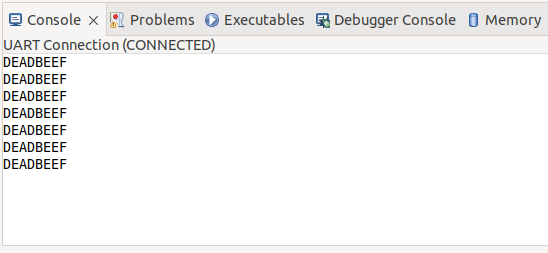
\includegraphics[width=0.7\textwidth]{anlagen/bilder/hw_test_uart}
    \caption{UART Monitorausgabe in der STMCubeIDE}
    \label{fig:impl-hw-uart-result}
\end{figure}

Die Funktionsweise des \ac{gpio}-Testprogramms ist aufgrund schlechter
Kameraverhältnisse nur schwer zu darzustellen.
Das Umschalten der LEDs ist mit bloßem Auge aber gut erkennbar.
\newline
Die Demo-Applikation des \ac{edi} Projekts konnte nicht auf dem
Entwicklungsboard ausgeführt werden.
Die \ac{hal} und \ac{cmsis} Bibliotheken konnte auf die CMake Konfiguration des
Demo Projekts übertragen werden.
Aufgrund der unerwartet hohen Komplexität und Unübersichtlichkeit der
\texttt{libopencm3} Bibliothek wird die Funktionsweise des \acl{edi} nur mit
der QEMU-Erweiterung dargestellt.
